Simulation of two-phase flow in porous media has applications in oil recovery, hydrology, electricity production where pressurised water is passed through heated pipes and is transformed into steam, etc. Hence it is important to understand and model two-phase flow in porous medium. \cite{labed2012experimental}

\subsection{Porous medium and capillary action}
	Figure \ref{fig_capillary_flow_brick} is an example of two-phase flow in porous media. The wetting fluid, in this case - water displaces the non wetting fluid - air, due to capillary action in the capillaries connecting the nodes, shown in figure \ref{fig_capact-of-water}.
	
	\begin{figure}[H]
		\centering
		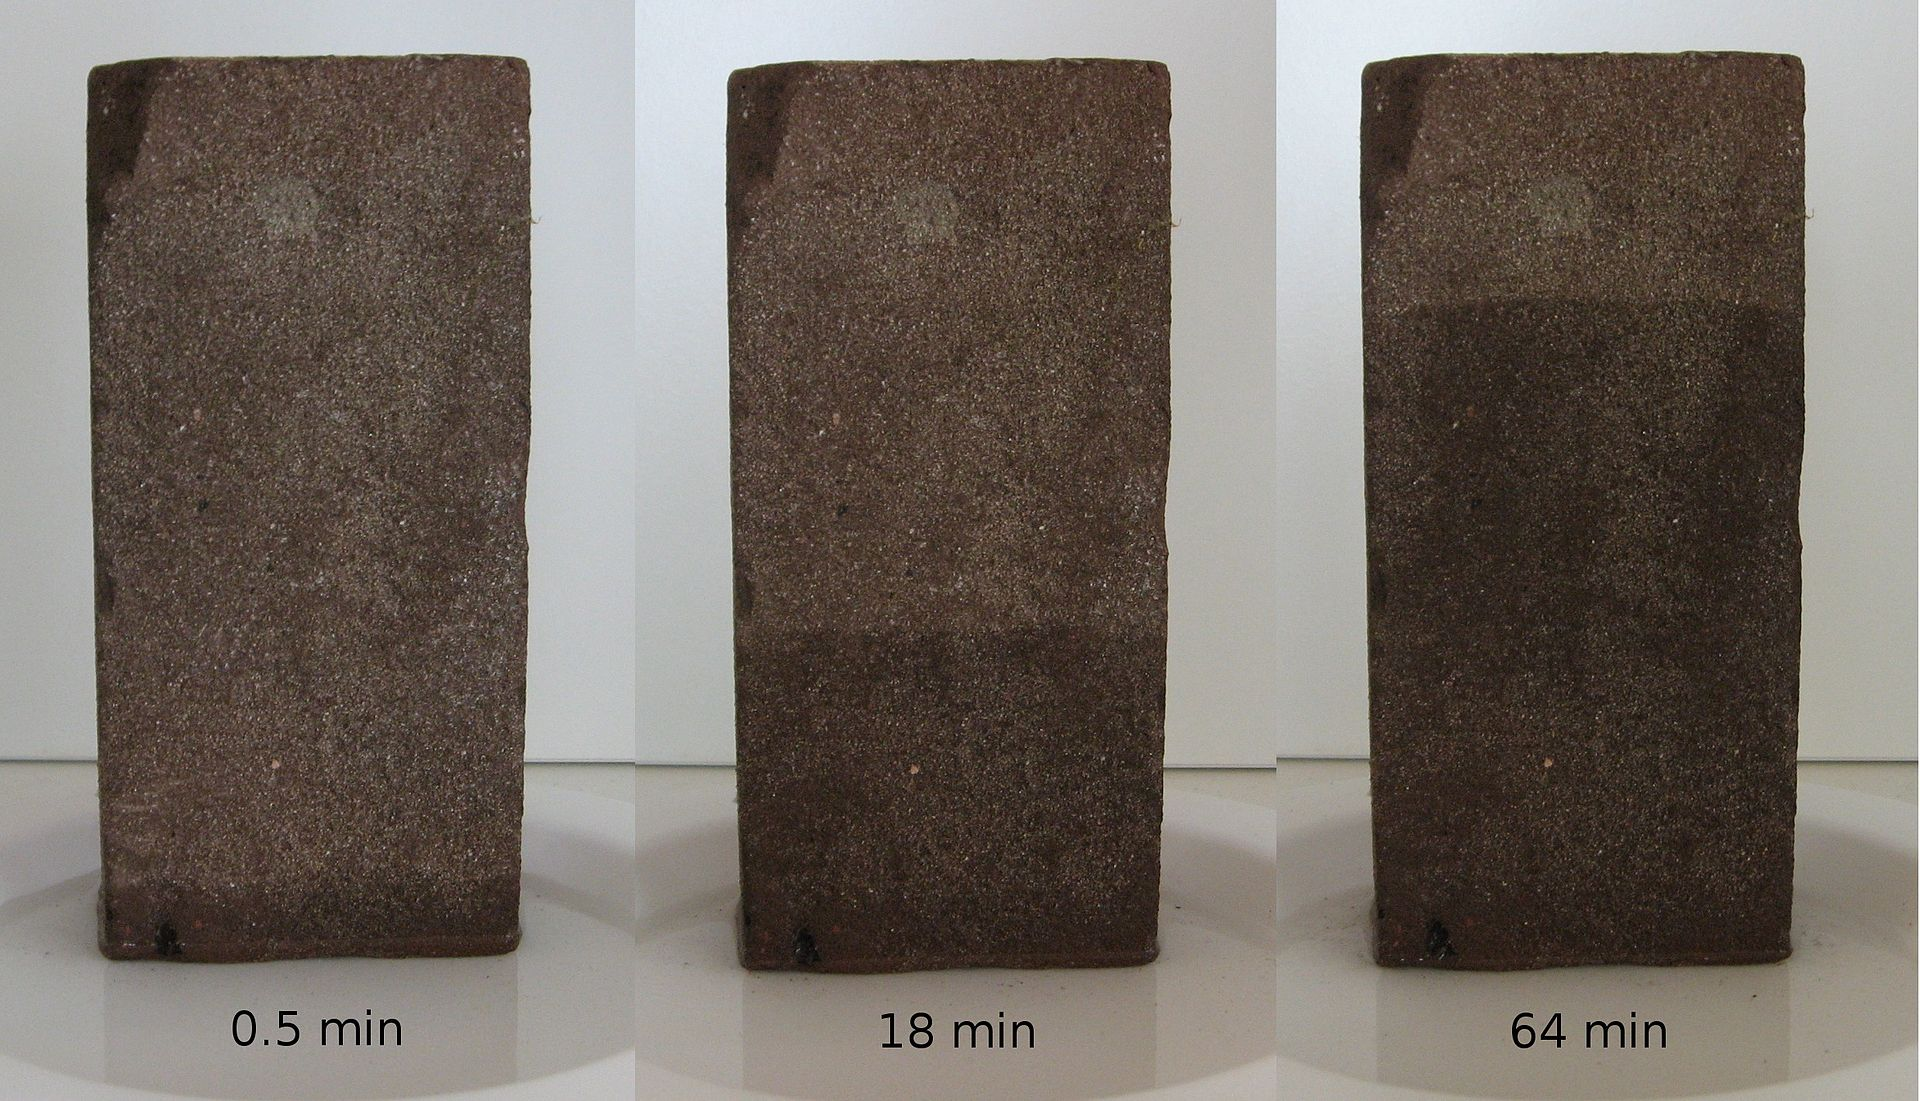
\includegraphics[width=0.8\textwidth]{fig_capillary_flow_brick}
		\caption{Water climbing against gravity through a porous medium due to capillary forces. \cite{wiki:Capillary_action}}
		\label{fig_capillary_flow_brick}
	\end{figure}
	
	\begin{figure}[H]
		\centering
		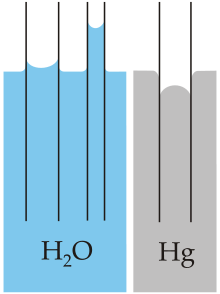
\includegraphics[width=0.3\textwidth]{fig_capact-of-water}
		\caption{Showing capillary action of water (polar) compared to mercury (non-polar), with respect to a polar surface such as glass (Si–OH). \cite{wiki:Capillary_action}}
		\label{fig_capact-of-water}
	\end{figure}
	
\subsection{Classical continuum models}

	Darcy's Law is a classical continuum model. It is given by:
	
	\begin{equation}
		q = -\frac{k}{\mu} \nabla p
		\label{eq:basic-darcy}
	\end{equation}
	
	Here, $q$ is the flow rate,	$k$ is the permeability, $\mu$ is the coefficient of viscosity,	$\nabla p$ is the pressure gradient.
	
	The feature of these classical continuum models is that the permeability is only a function of the saturation of one of the phase.
	\begin{equation}
		k = k(S)
	\end{equation}
	
	Here, $k$ is the permeability as in equation \ref{eq:basic-darcy}, $S$ is the saturation of one of the phase.

	Saturation $S$ is defined as the ratio between the volume occupied by a phase to the total volume of the void.

	\begin{equation}
		S = \frac{V_{w}}{V_{void}}
	\end{equation}
	
	Here, $V_{w}$ is volume occupied by the wetting phase, $V_{void}$ is total volume of the void.
	
\subsection{Advanced continuum models}
	The classical continuum models are valid as long as the characteristic time of the processes is much longer than the characteristic time of fluid redistribution in the capillary space.
	
	When the saturation changes rapidly, or the porous medium has a structure such that the time of fluid redistribution is long. For example in fractured-porous medium with blocks and cracks, the assumption that $k = k(S)$ is not sufficient and additional parameters are required.

	Various advanced continuum models that take these effects into account. Models of Hassanizadeh \cite{hassanizadeh2004continuum} \cite{hassanizadeh1987high} and Barenblatt \cite{barenblatt1960basic} consider that, the permeability $k$ is a function of the rate of saturation change $\frac{\partial S}{\partial t}$ in addition to the saturation $S$.                  
	
	\begin{equation}
		S = S(t)
	\end{equation}
		
	\begin{equation}
		k = k(S, \frac{\partial S}{\partial t})
	\end{equation}
	
	The Kondaurov model \cite{kondaurov2009non} considers a special non-equilibrium parameter $\xi$ along with saturation $S$, which relaxes to an equilibrium value. \cite{kondaurov2007thermodynamically}
	
	\begin{equation}
		k = k(S, \xi)
	\end{equation}
	
	This parameter $\xi$ is related to $S$ by the differential equation:
	
	\begin{equation}
		\frac{\partial \xi}{\partial t} = \Omega ( S, \xi )
	\end{equation}
	
	The final objective of our network model is to understand the physical meaning of the non-equilibrium parameter $\xi$.
	 
\subsection{Non-continuum models}
	It is necessary to simulate the flow at the scale of pores, in order to better understand the non-equilibrium characteristics. Lattice Boltzmann Method, direct Navier-Stokes simulation or a network model are some of the methods of modelling at the scale of pores. Direct Navier-Stokes simulation provides but is very complicated. Network models are much simpler to model and perform computations than direct Navier–Stokes calculations.
	
	One of the earliest models simulated the flow using a network of electrical resistors \cite{fatt1956network}. Some of the modern models simulated using hour glass shaped model of tubes \cite{aker1998two}, where the average flow rate is given by the Washburn equation for capillary flow \cite{washburn1921dynamics}, the disadvantage is that the flow rate must be approximated for cylindrical tube while in the model, the capillary pressure varies depending on its position in the tube.
	
	The network model we developed uses cylindrical tubes, the flow rate is given by simple equations, also made use of a new method for distributing phases at the nodes. The applicability of our model in this article is shown by modelling imbibition.
